\documentclass{standalone}
\usepackage{tikz}
\usetikzlibrary{arrows,calc}

\begin{document}

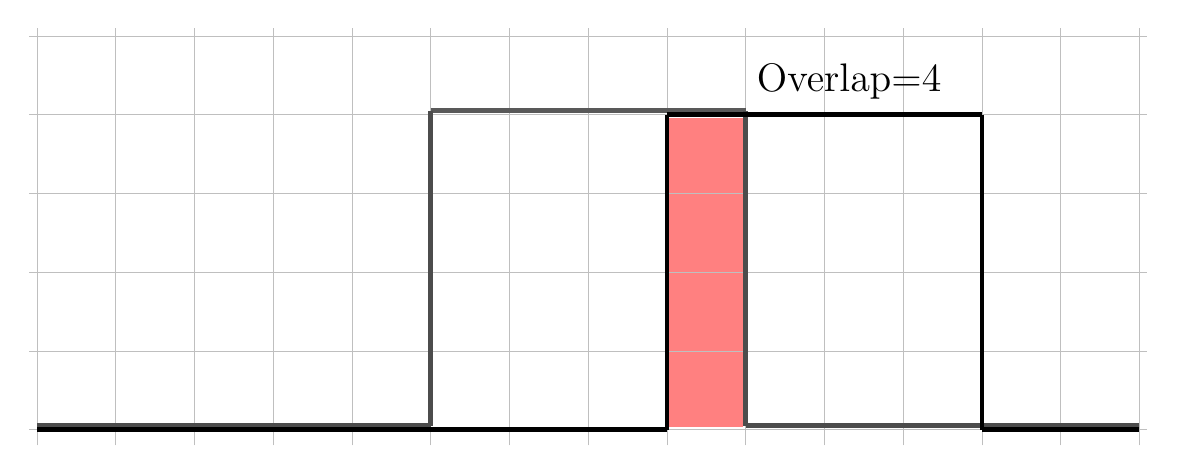
\begin{tikzpicture}

  \fill [red!50] (1.03,0.03) rectangle (1.97,3.96);
    \draw[very thin,color=gray!50] (-7.1,-0.2) grid (7.1,5.1);

    \draw[-,ultra thick, color=black!65] (-2,4.05) --
    (2,4.05) node[above right,
    color=black, font = \Large] {Overlap=4} ;
    \draw[-,ultra thick, color=black!70] (-2,0.05) -- (-2,4.05) node[above] {};
    \draw[-,ultra thick, color=black!70] (2,0.05) -- (2,4.05) node[above] {};
    \draw[-,ultra thick, color=black!70] (2,0.05) -- (7,0.05) node[above] {};
    \draw[-,ultra thick, color=black!70] (-2,0.05) -- (-7,0.05) node[above] {};

    \draw[-,ultra thick] (1,4) -- (5,4) node[above] {};
    \draw[-,ultra thick] (1,0) -- (1,4) node[above] {};
    \draw[-,ultra thick] (5,0) -- (5,4) node[above] {};
    \draw[-,ultra thick] (5,0) -- (7,0) node[above] {};
    \draw[-,ultra thick] (1,0) -- (-7,0) node[above] {};

\end{tikzpicture}
\end{document} 
